\section{Studies} % (fold)
\label{sec:studies}

To begin understanding what a deep network can learn about jet topology, we choose a finite region of phase space, and standardize our comparisons. In an effort to define a standard way that physics object identification using machine learning should be conducted, we exactly define our procedure for comparisons. In particular, we restrict our studies to $250$ GeV $\leq p_T \leq 300$ GeV, and confine ourselves to a $65$ GeV $\leq m \leq 95$ GeV mass window, wholly containing the peak of the $W$. 

We construct a scaffolded and multi-approach series of methodologies for understanding, visualizing, and validating neural networks within HEP.

\subsection{Figure of Merit} % (fold)
\label{sec:figure_of_merit}

As is commonly done in High Energy Physics, we eschew the commonly chosen metric of basic accuracy in favor of the Receiver Operating characteristic. This is because we must examine the entire spectrum of trade-off between Type-I and Type-II error, as many applications in physics will choose different points along the trade-off curve. We use a slight modification of the traditional ROC. For any discriminating variable, let $c$ be a threshold on the likelihood ratio on that variable, and let $w$ be the vector of weights over the entire evaluation sample. We define the \emph{rejection} of such a threshold is defined as 
$$
    \rho(c) = \frac{1}{\text{FPR}(c, w)},
$$
where $\text{FPR}(c, w)$ is the weighted false positive rate for using $c$ as a threshold.

We define the \emph{efficiency} of $c$ as 
$$
    \varepsilon(c) = \text{TPR}(c, w),
$$
where $\text{TPR}(c, w)$ is the weighted false positive rate for using $c$ as a threshold. We then evaluate our algorithms using the area under the line generated by $\{(\varepsilon(c), \rho(c)) : \varepsilon(c)\in [0.2, 0.8]\}$. We say that an classifier is \emph{strictly} more performant if the ROC curve is above a baseline for all efficiencies.



\subsection{Coarse Studies} % (fold)
\label{sub:coarse_studies}

To a first order, the first desirable characteristic is a simple performance improvement over the standard physics-driven variables for discrimination. In particular, we compare our network to $n$-subjettiness~\cite{nsub} and the jet mass. We henceforth refer to $n$-subjettiness as $\tau_{21}$ for our purposes, as $\tau_{2}/\tau_{1}$ is relevant for our classification problem.

In Figure~\ref{fig:combinedROC}, we illustrate the performance gains of a deep neural network over both $\tau_{21}$ and the 2D likelihood of $\tau_{21}$ and jet mass. 


\begin{figure}[!htbp]
  \centering
  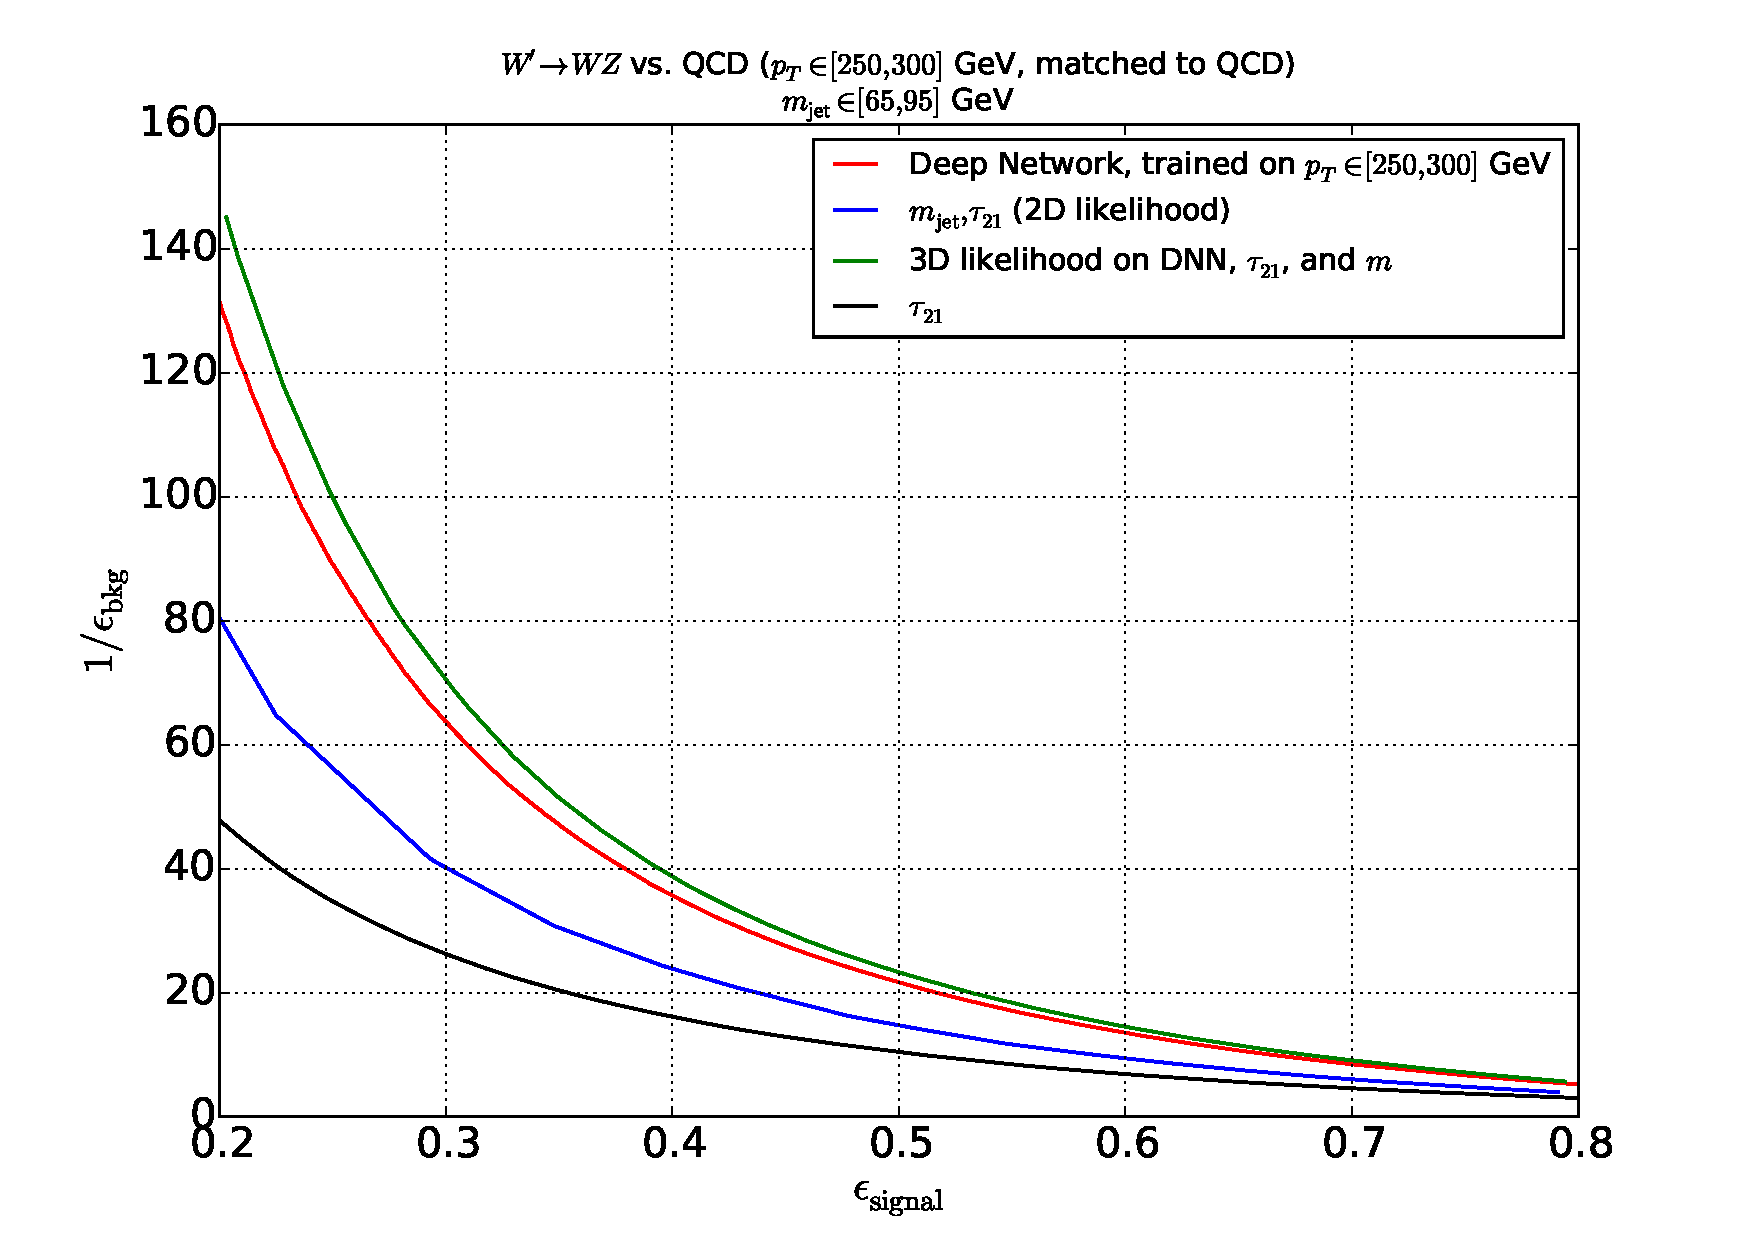
\includegraphics[width=0.95\textwidth]{figures/combined-roc.pdf}
  \caption{Receiver Operating Characteristic (ROC) over coarse sample}
  \label{fig:combinedROC}
\end{figure}

We also provide a comparison to a 3D likelihood constructed on $\tau_{21}$, jet mass, and the deep network output itself. We can gain a significant piece of insight from this. Note how in Figure~\ref{fig:combinedROC} we can see that the DNN represents a large gain on a physics-only likelihood. However, when we explicitly include the physics variable in a 3D likelihood, we see a small but definitively non-zero performance gain. This implies that the performance boost \emph{by definition} is getting its gain from something that is not \emph{fully} encapsulated in $\tau_{21}$ and jet mass. 

Though important on it's own, this figure of merit does little to help drive understanding in the context of HEP. Such an increase begs further questions -- what is this gain, and where does it come from? Why is the DNN able to pick up on this?



\subsubsection{Understanding what is learned} % (fold)
\label{ssub:understanding_what_is_learned}

% subsubsection understanding_what_is_learned (end)
In Figure~\ref{fig:convkernels}, we first examine the $11\times11$ convolutional filters in the first layer and look for structure. In

In order to understand what we learn, we first take a look \emph{inside} the deep network, and visualize features learned during training.

\begin{figure}[bt]
  \begin{center}
      \subfloat[$(11\times11)$ convolutional kernels from first layer \label{subfig:filters}]{
        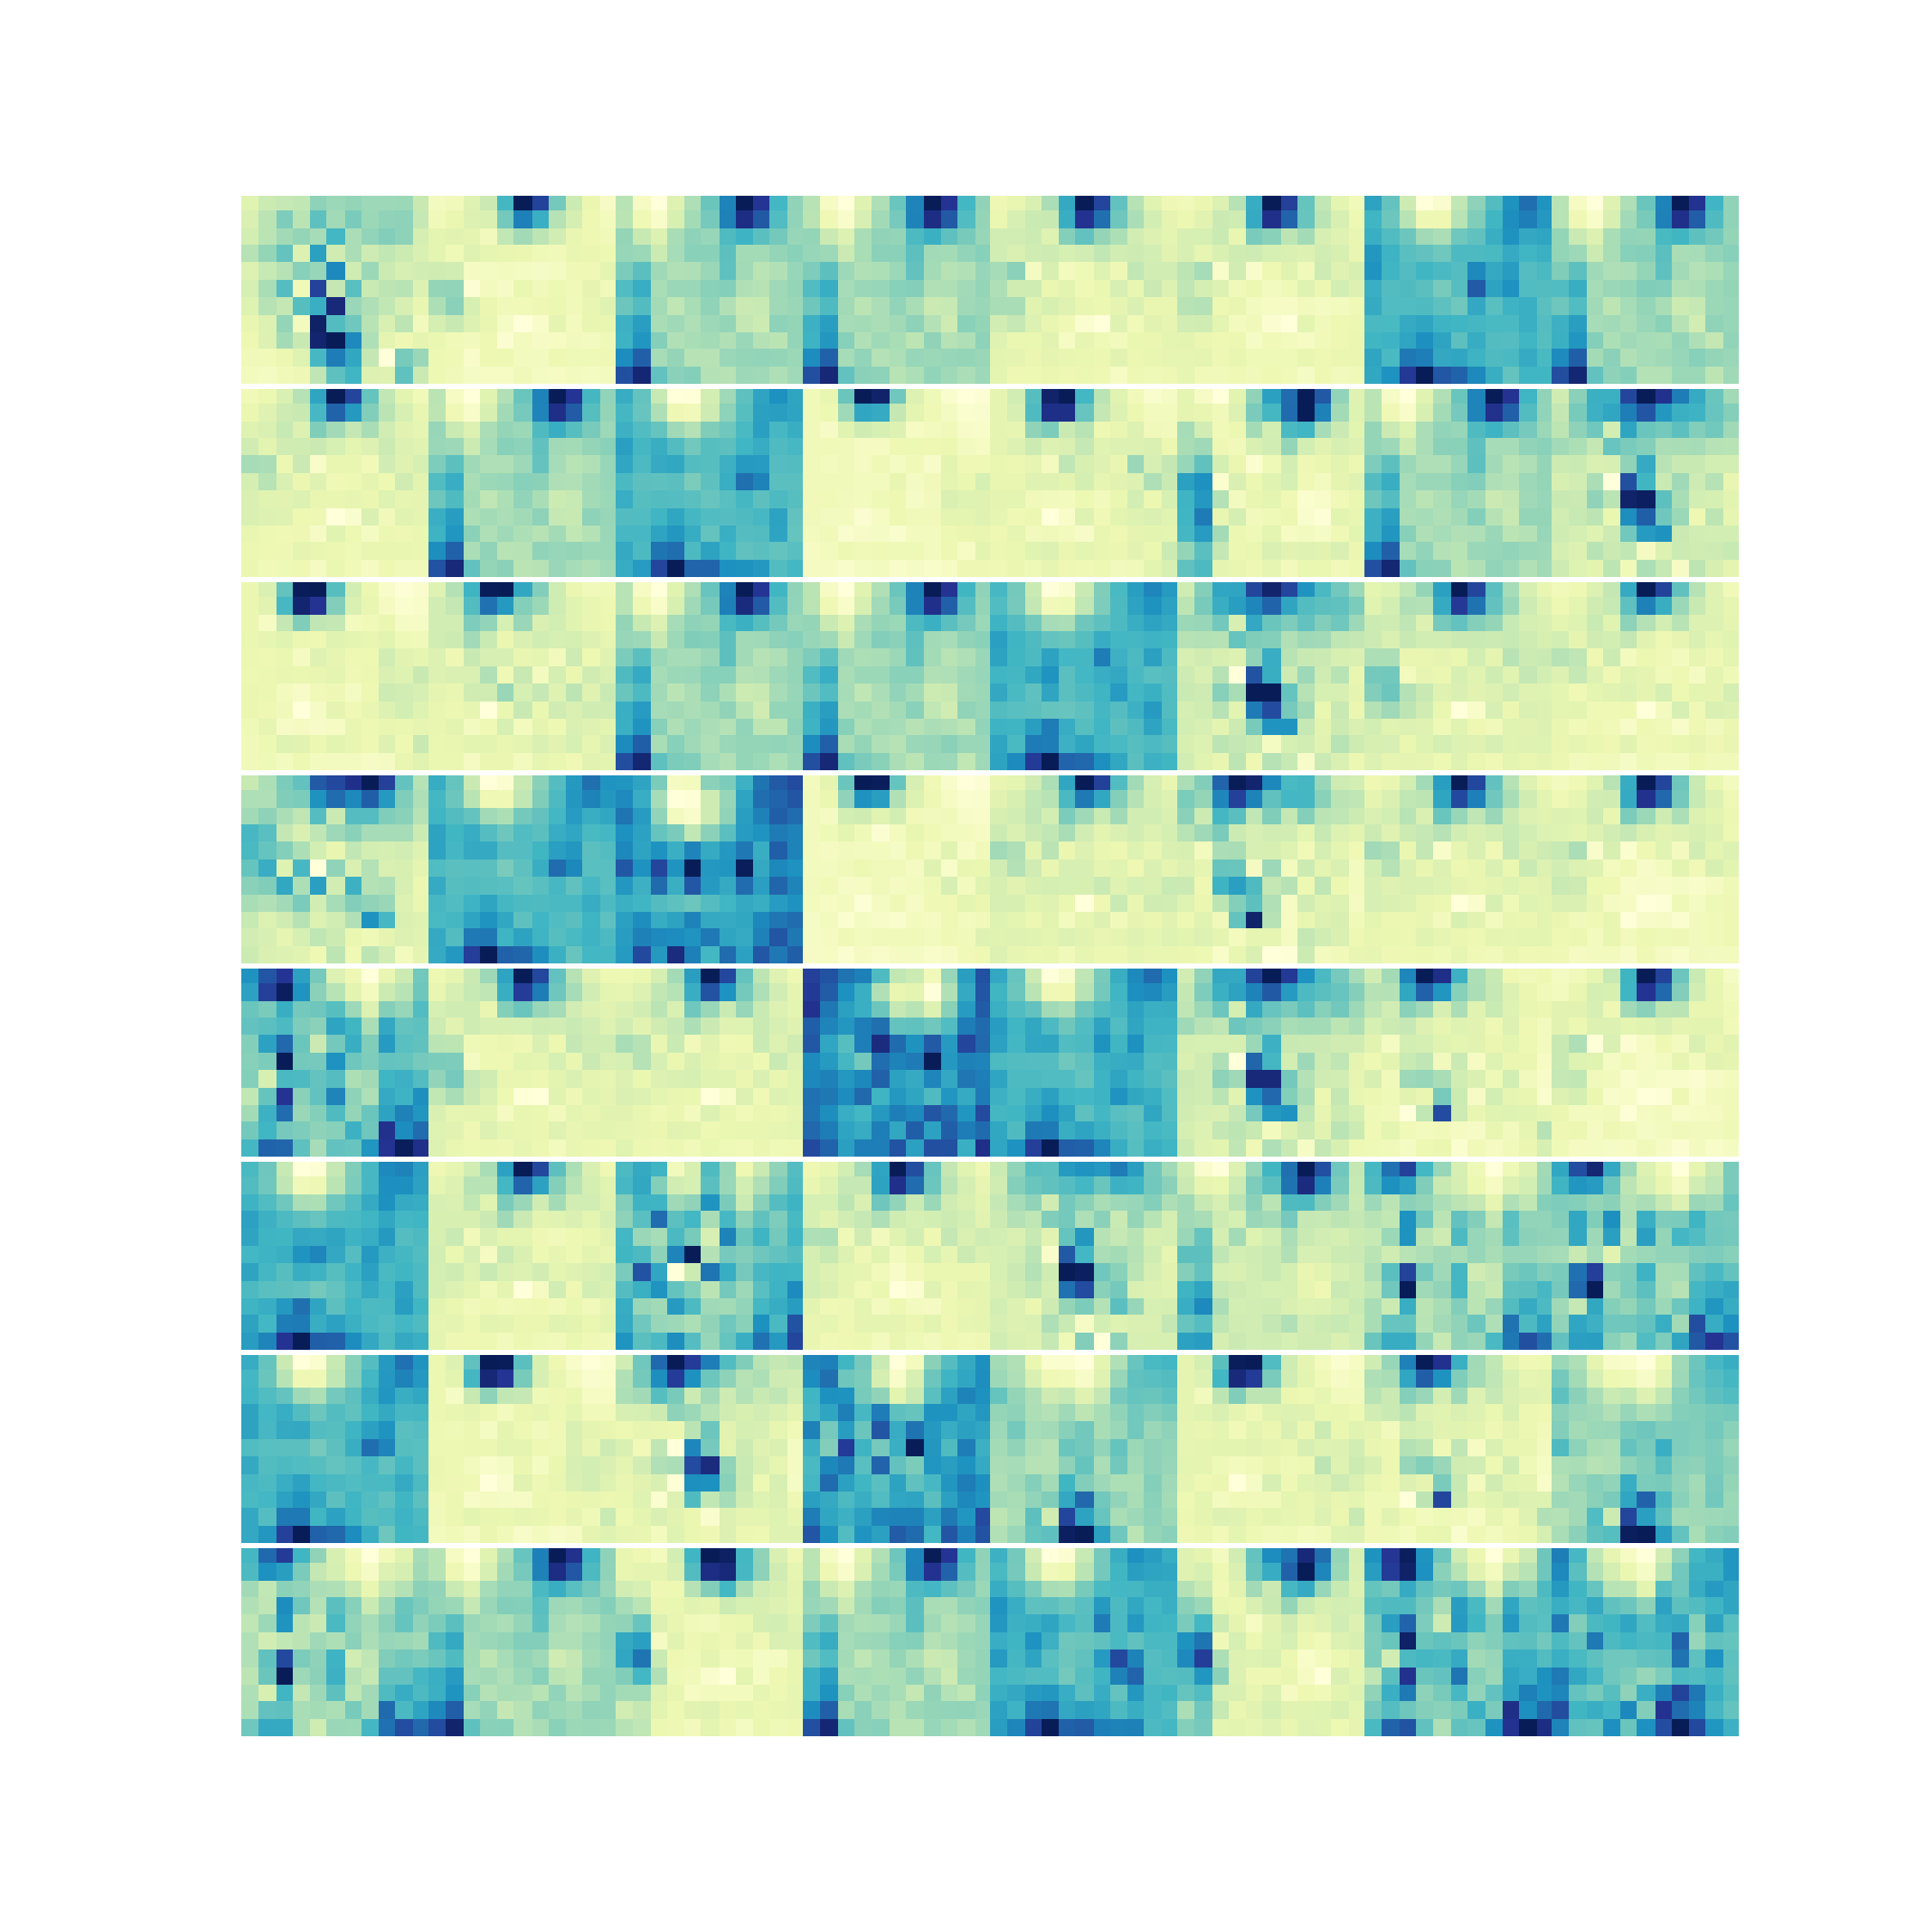
\includegraphics[width=0.5\textwidth]{figures/conv-filts.pdf}
      }
      \subfloat[Convolved Jet Image differences\label{subfig:convolvedfilters}]{
        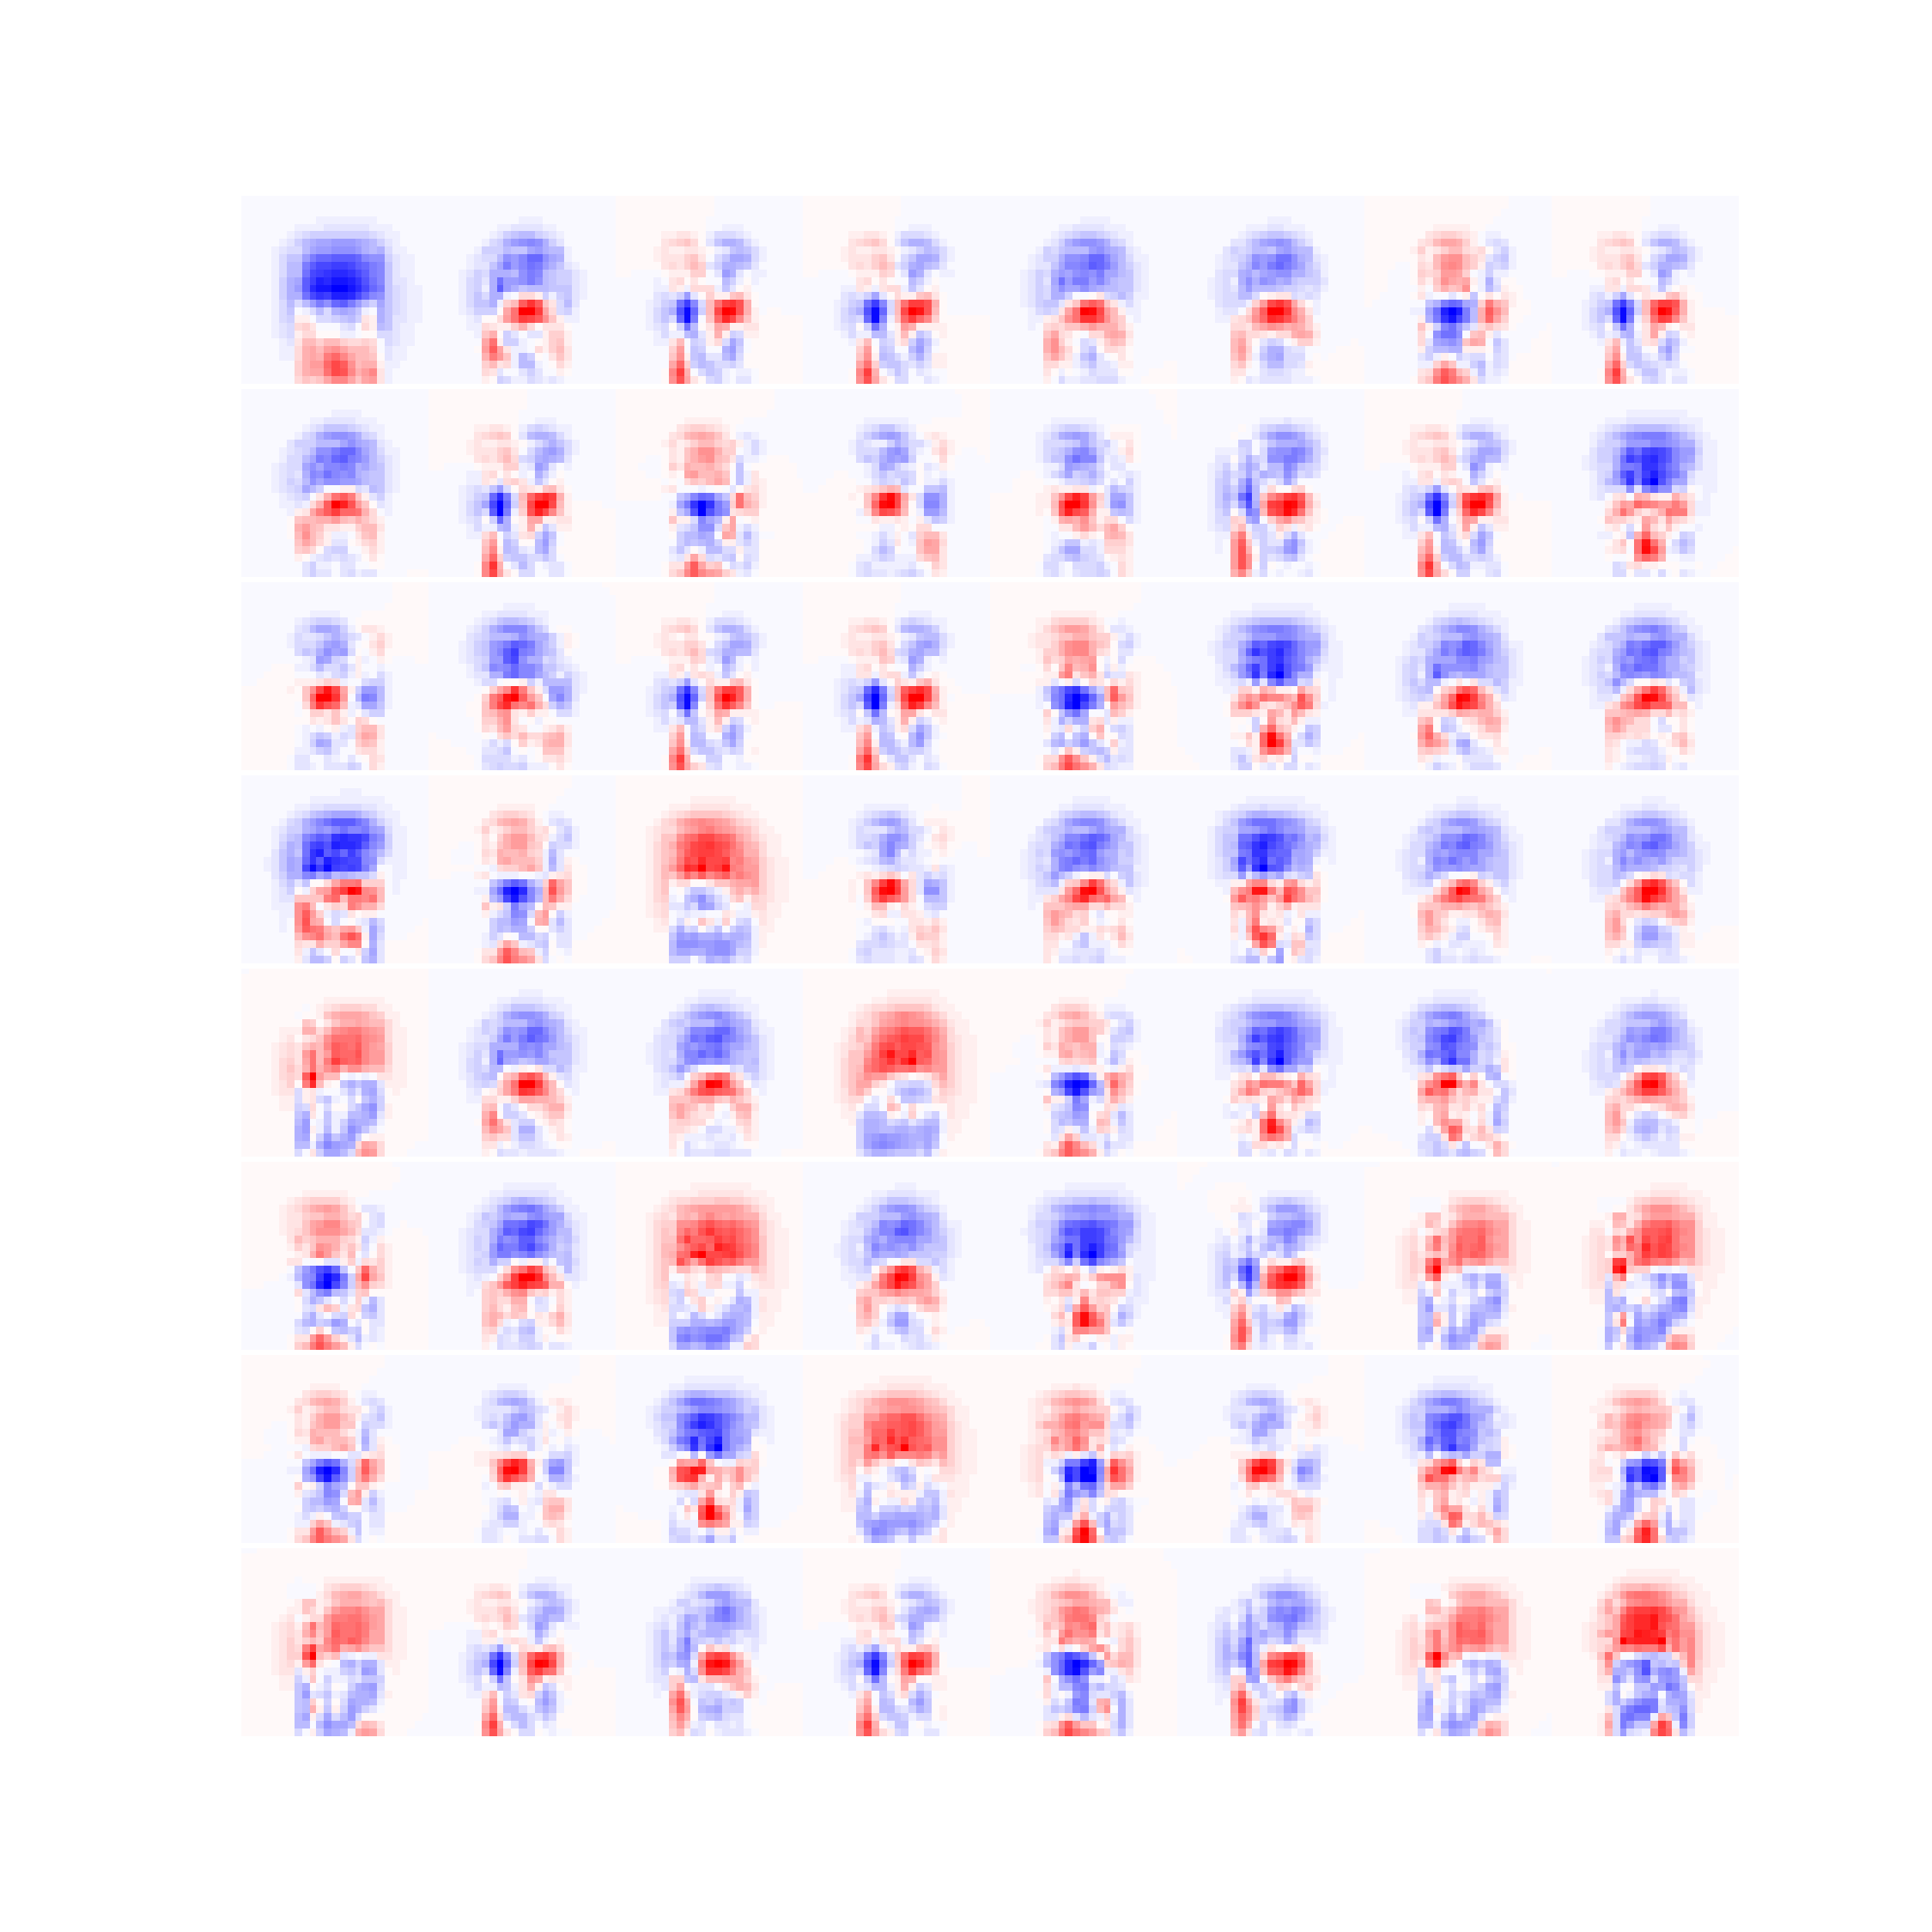
\includegraphics[width=0.5\textwidth]{figures/conv-diffs-global.pdf}
      }
      \caption{Convolutional Kernels (left), and convolved feature differences in jet images (right)}
      \label{fig:convkernels}

    \end{center}
\end{figure}

In Figure~\ref{subfig:filters}, we show the (11$\times$11) convolutional filters learned by our network. To mimic the operation in the first layer of the network, we can convolve each filter with an average jet image to get an understanding of what features the network learns at the first layer. 

More formally, let $J_s=\frac{1}{n}\sum_{i:i\text{ is signal}} J^{(i)}$ and $J_b=\frac{1}{n}\sum_{i:i\text{ is background}}J^{(i)}$ represent the average signal and background jet over a sample, where $J^{(i)}$ is the $i$th jet image. In addition, we can select a filter $w_i\in\mathbb{R}^{11\times11}$ from the first convolutional layer.

We then examine the differences in the post convolution layer. We take 

\begin{equation}
  J_s \ast w_i - J_b \ast w_i, \forall i,
\end{equation}

where $\ast$ is the standard convolution operator. We arrange these new ``convolved images'' in a grid, and show in red regions where signal has a stronger representation, and in blue where background has a stronger representation. In Figure~\ref{subfig:convolvedfilters}, we show the convolved differences described above, where each $(i, j)$ image is the representation under the $(i, j)$ convolutional filter. We note the existence of interesting patterns around the regions where the leading and subleading subjets are expected to be. We also draw attention to the fact that there is a large diversity in the the convolved representations, indicating that the DNN is able to learn and pick up on multiple features that are descriptive.



\subsubsection{Physics in Deep Representations} % (fold)
\label{ssub:physics_in_deep_representations}

To get a tangible and more intuitive understanding of what jet structures a DNN learns, we construct the following. Let $y$ be the DNN output, and consider every pixel $p_ij$ in transformed $(\eta, \phi)$ space. We the construct an image where each pixel $(i, j)$ is $\rho_{p_{ij}, y}$, the Pearson Correlation Coefficient of that pixels energy deposition with the final DNN output. In Figure~\ref{fig:corr}, we construct this image, and can see interesting structure in the subleading subjet region as well as asymmetric scattering patterns around the leading subjet.




\begin{figure}[!htbp]
  \centering
  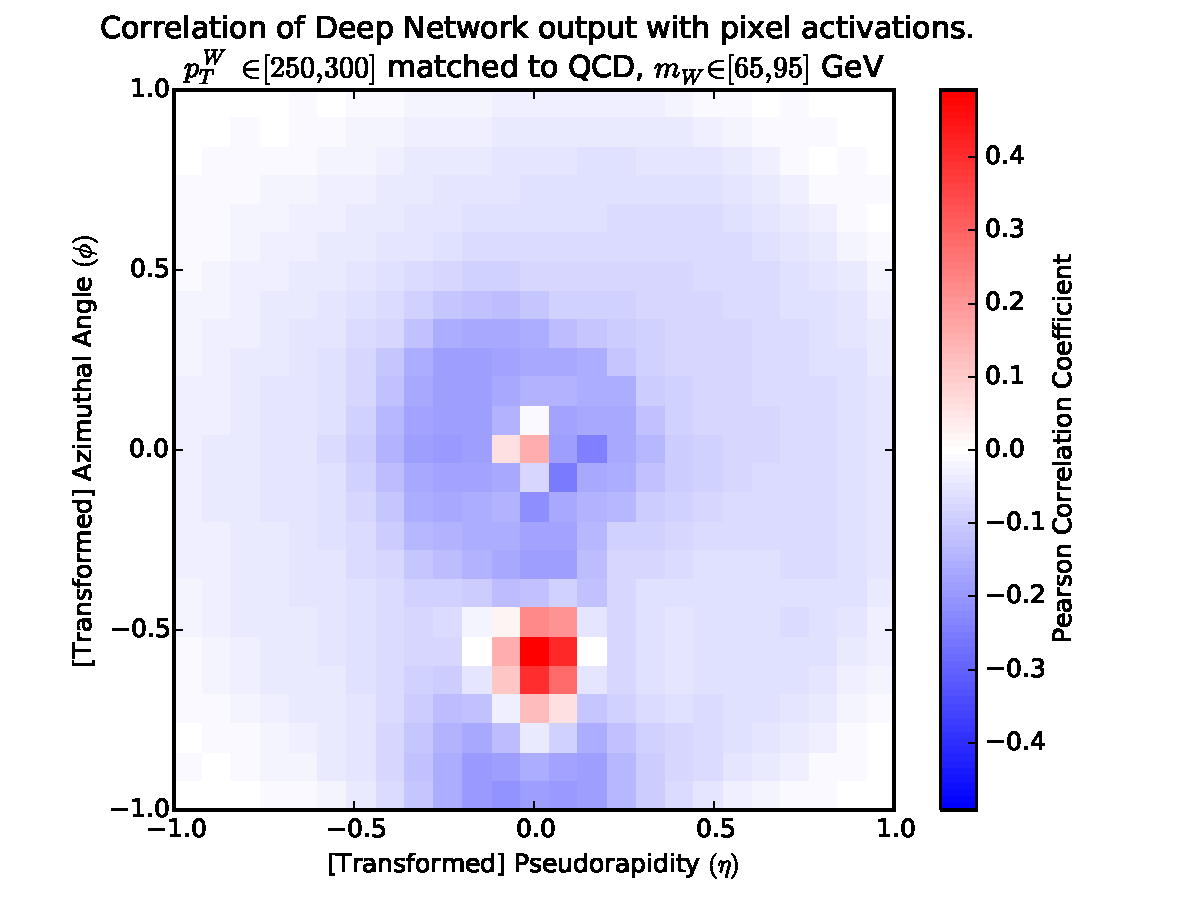
\includegraphics[width=0.95\textwidth]{figures/pixel-activations-corr.pdf}
  \caption{Per-pixel linear correlation with DNN output}
  \label{fig:corr}
\end{figure}


\begin{figure}[bt]
  \begin{center}
      \subfloat[Sculpted QCD $\Delta R$ distribution\label{fig:sculpteddR}]
      {
        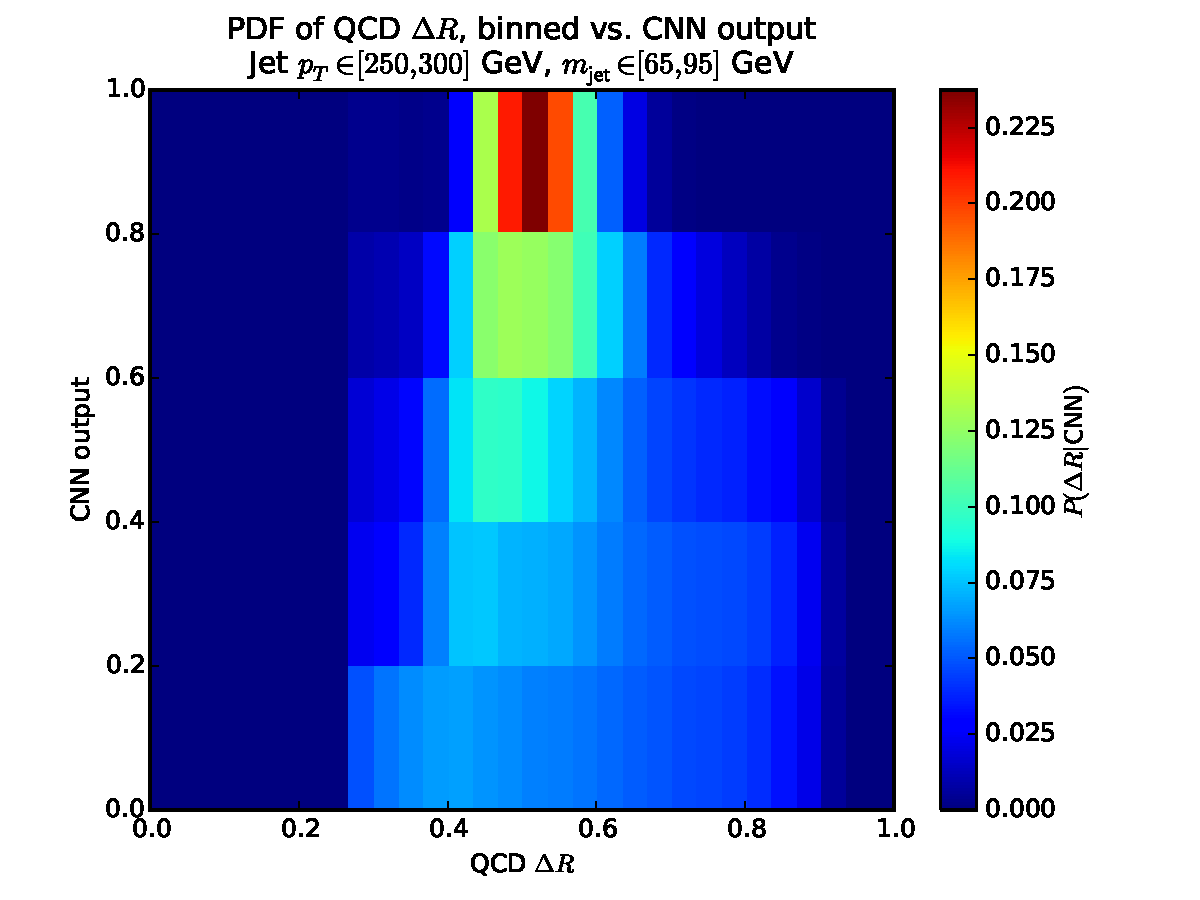
\includegraphics[width=0.5\textwidth]{figures/dR-dist-by-CNN.pdf}
      }
      \subfloat[Sculpted QCD $\tau_{21}$ distribution\label{fig:sculptednsj}]
      {
        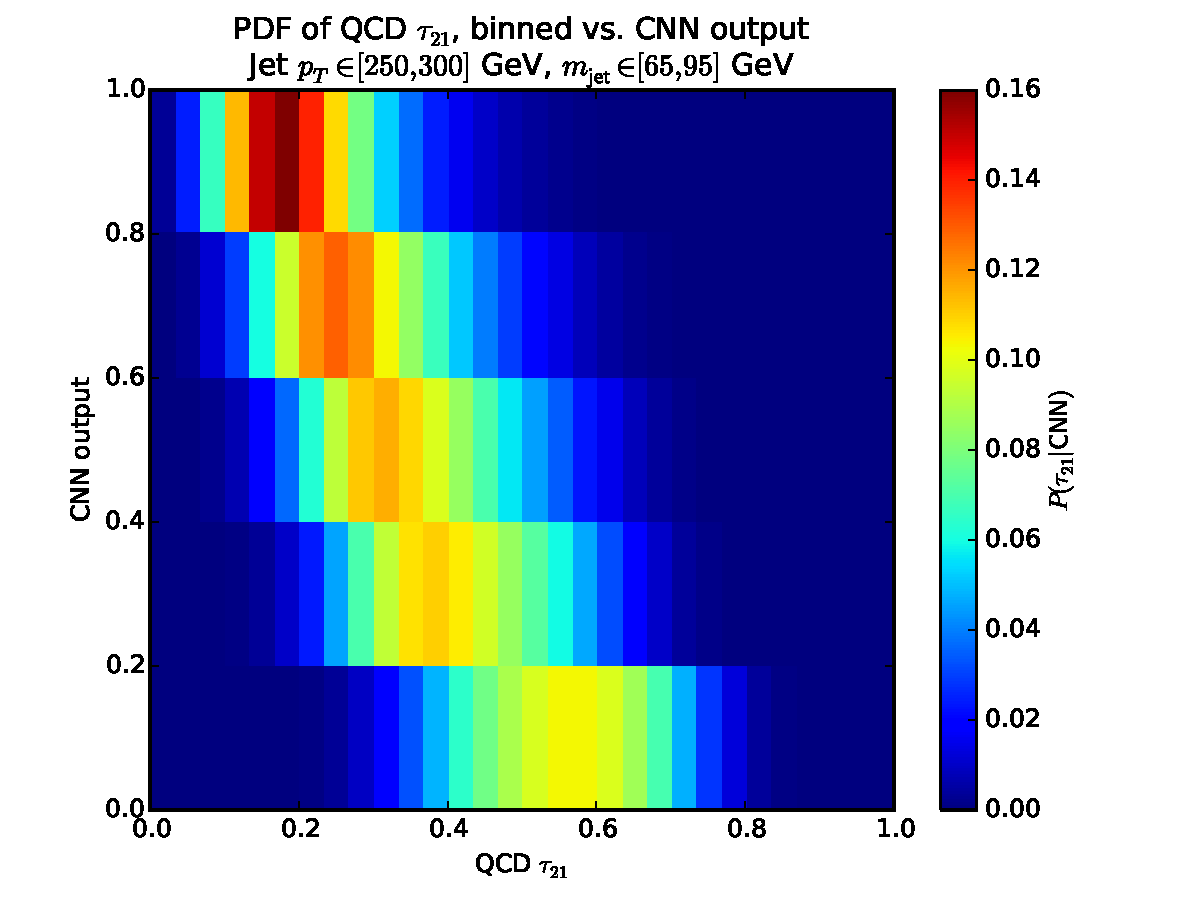
\includegraphics[width=0.5\textwidth]{figures/tau-dist-by-CNN.pdf}
      }
      \\
      \subfloat[Sculpted QCD mass distribution\label{fig:sculptedmass}]
      {
        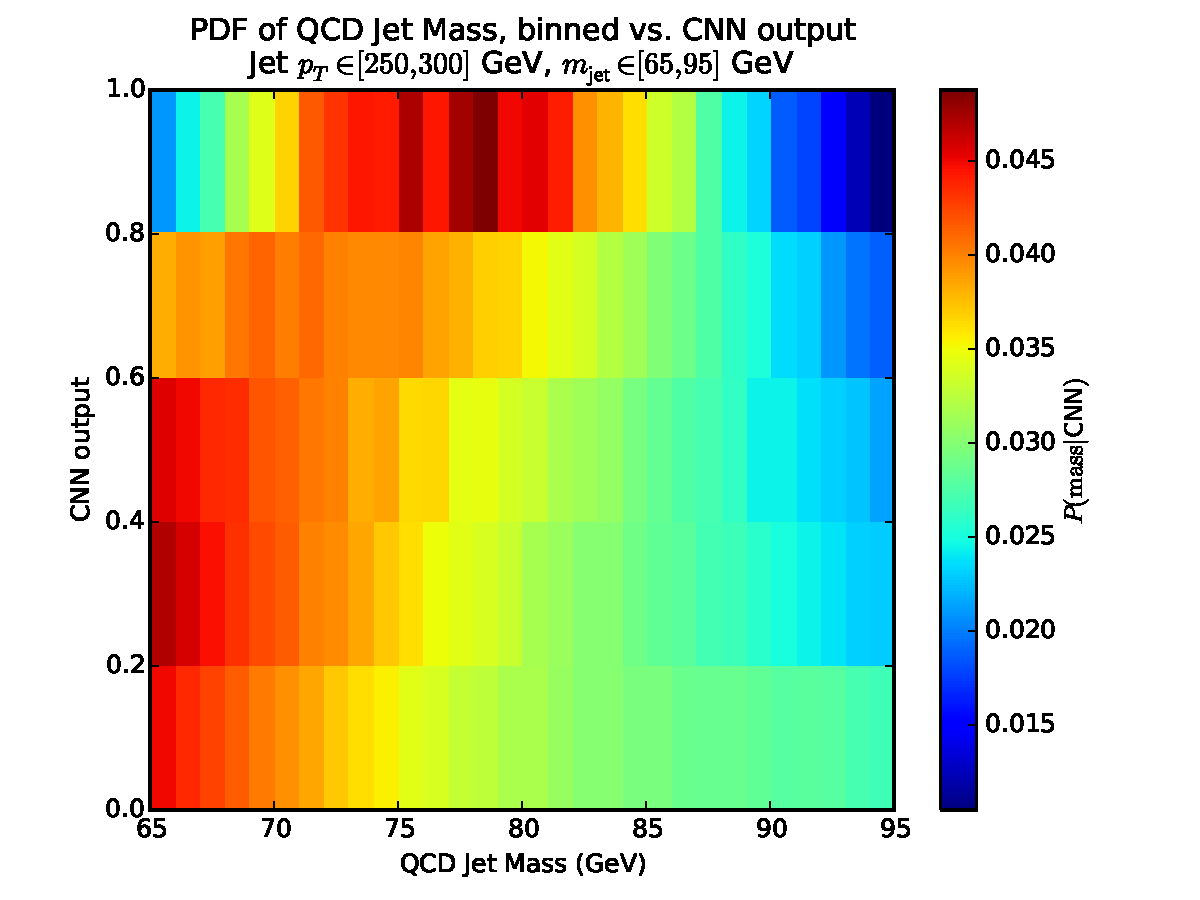
\includegraphics[width=0.5\textwidth]{figures/mass-dist-by-CNN.pdf}
      }

      \caption{Sculpted QCD distributions}
      \label{fig:qcdsculpt}

    \end{center}
\end{figure}





% subsubsection physics_in_deep_representations (end)

% subsection coarse_studies (end)

\subsection{Flat Hypercube Studies} % (fold)
\label{sub:flat_hypercube_studies}

Since we outperform physics-derived variables, we would like to know where these performance improvements come from. Our first approach to this is \emph{hypercube reweighting}. In particular, we derive weights such that the joint distributions of mass, $n$-subjettiness, and $p_T$ are non-discriminative. Specifically, we require

\begin{equation}
  f(m, \tau_{21}, p_T| W'\rightarrow WZ) \approx f(m, \tau_{21}, p_T| QCD).
\end{equation}

We then take our globally trained neural network (Figure~\ref{fig:combinedROC}) and apply the discriminant under this ``flattening'' transformation. We also use the training weights inside this window and train an additional CNN. In particular, we look for increases in performance, which would indicate information learned beyond physics variables since we removed the discrimination power using hypercube weighting.

In Figure~\ref{fig:rocCube} we show that the globally trained NN retains discrimination power even once we ``subtract'' the discrimination power of primitives from physics.

\begin{figure}[htbp]
  \centering
  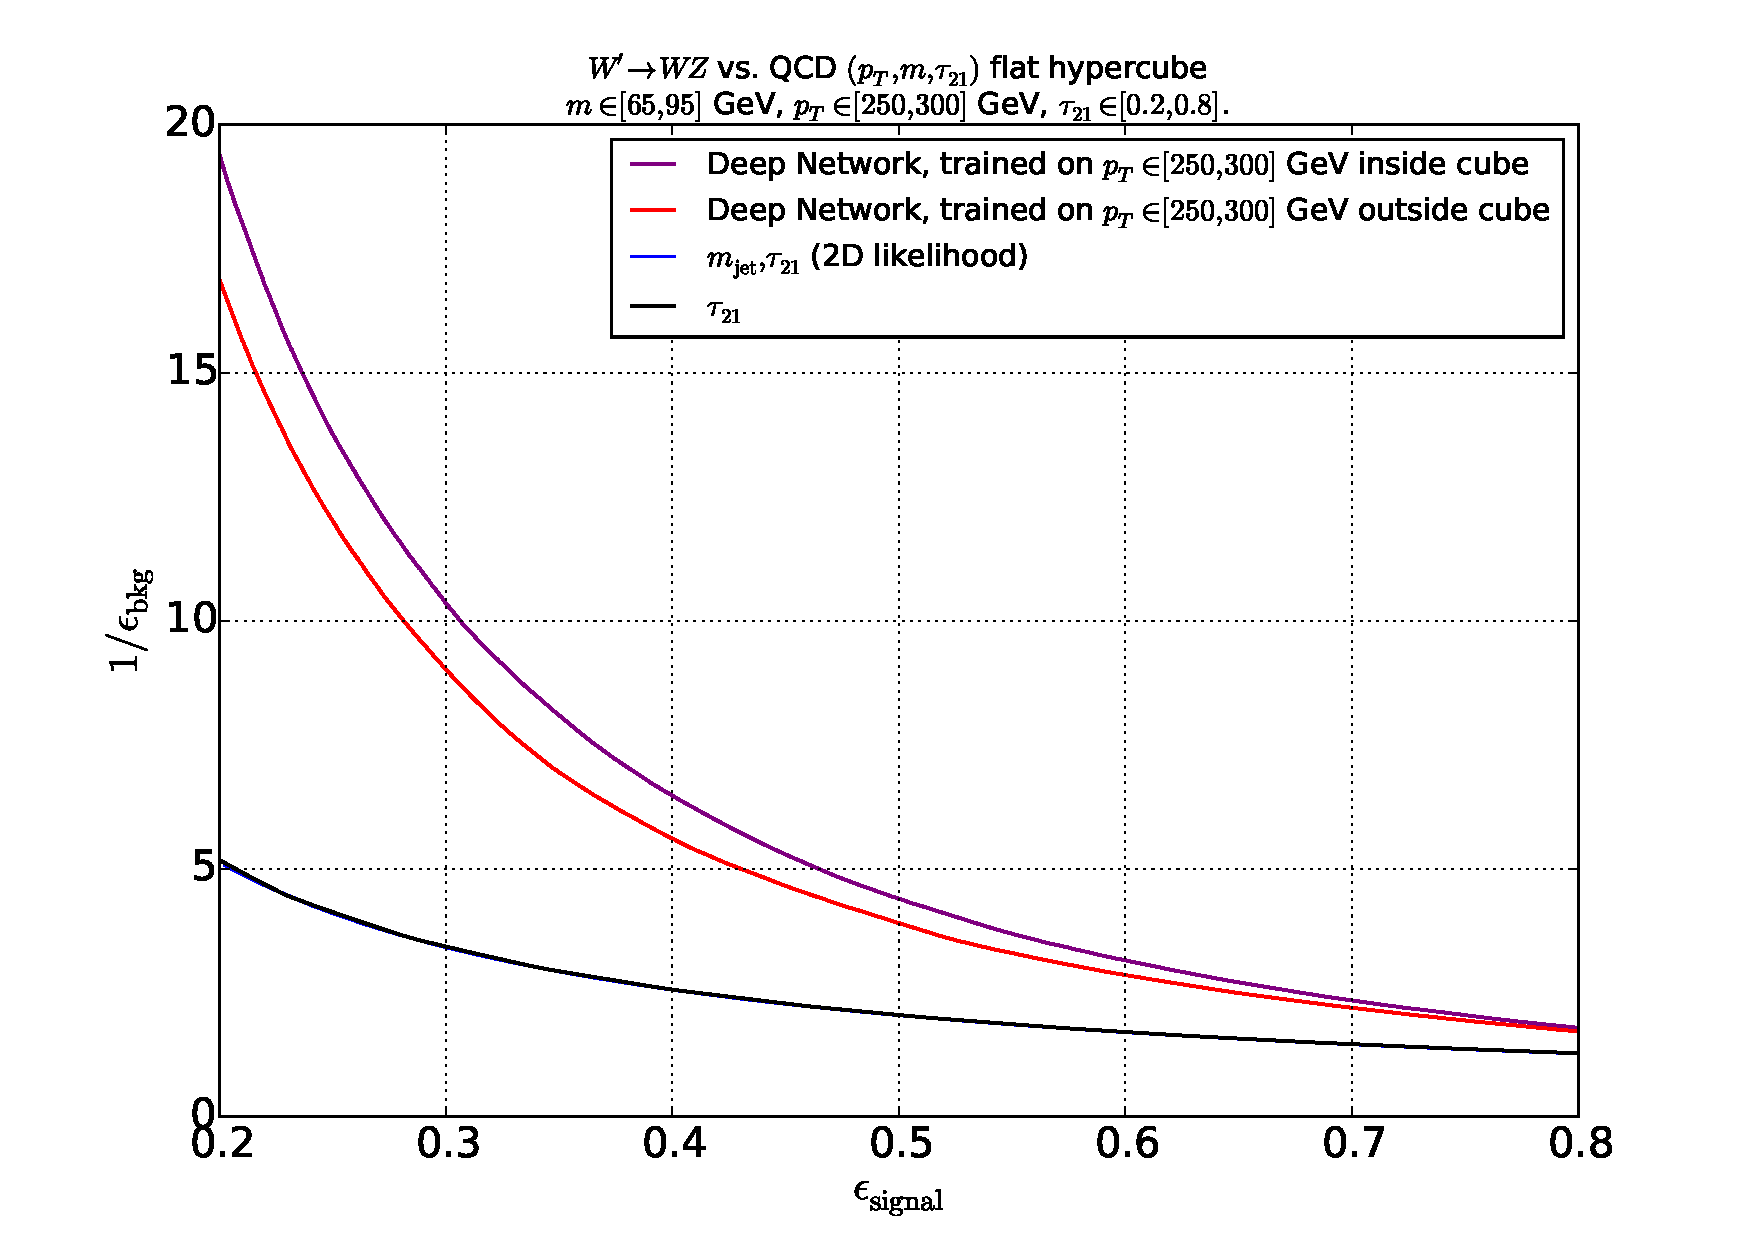
\includegraphics[width=0.95\textwidth]{figures/roc-cube-inside.pdf}
  \caption{ROC Curve for weigth-flattened hypercube, with $m\in[65, 95]\mathsf{GeV}$,  $p_T\in[250, 300]\mathsf{GeV}$, and  $\tau_{21}\in[0.2, 0.8]$}
  \label{fig:rocCube}
\end{figure}

% subsection flat_hypercube_studies (end)



\subsection{Small Window Studies} % (fold)
\label{sub:small_window_studies}

Though we see performance improvements using a deep network under an induced flat hypercube, we want to be sure that these performance improvements are valid and carry over to a less contrived distribution. In particular, we consider a mass window of [79, 81] GeV, a $p_T$ window of [250, 255] GeV, and we require $\tau_21$ to be in [0.19, 0.21]. In Figure~\ref{fig:meanImagesWindow}, we see the differences between signal and background for such a window.

\begin{figure}[bt]
  \begin{center}
  
      \subfloat[Average $W'\rightarrow WZ$ image \label{subfig:sig_window}]{
        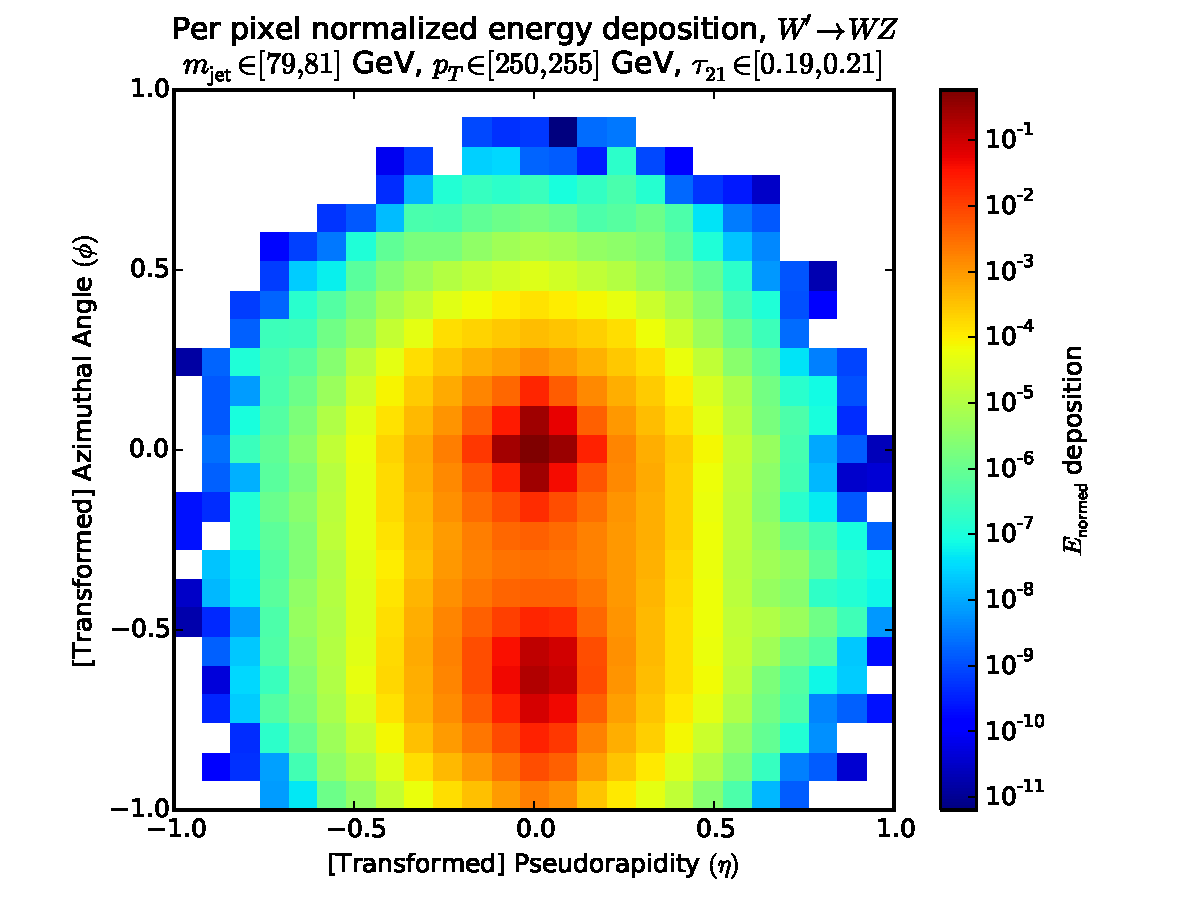
\includegraphics[width=0.5\textwidth]{figures/avg-benwindow-sig.pdf}
      }
      \subfloat[Average QCD image \label{subfig:bkg_window}]{
        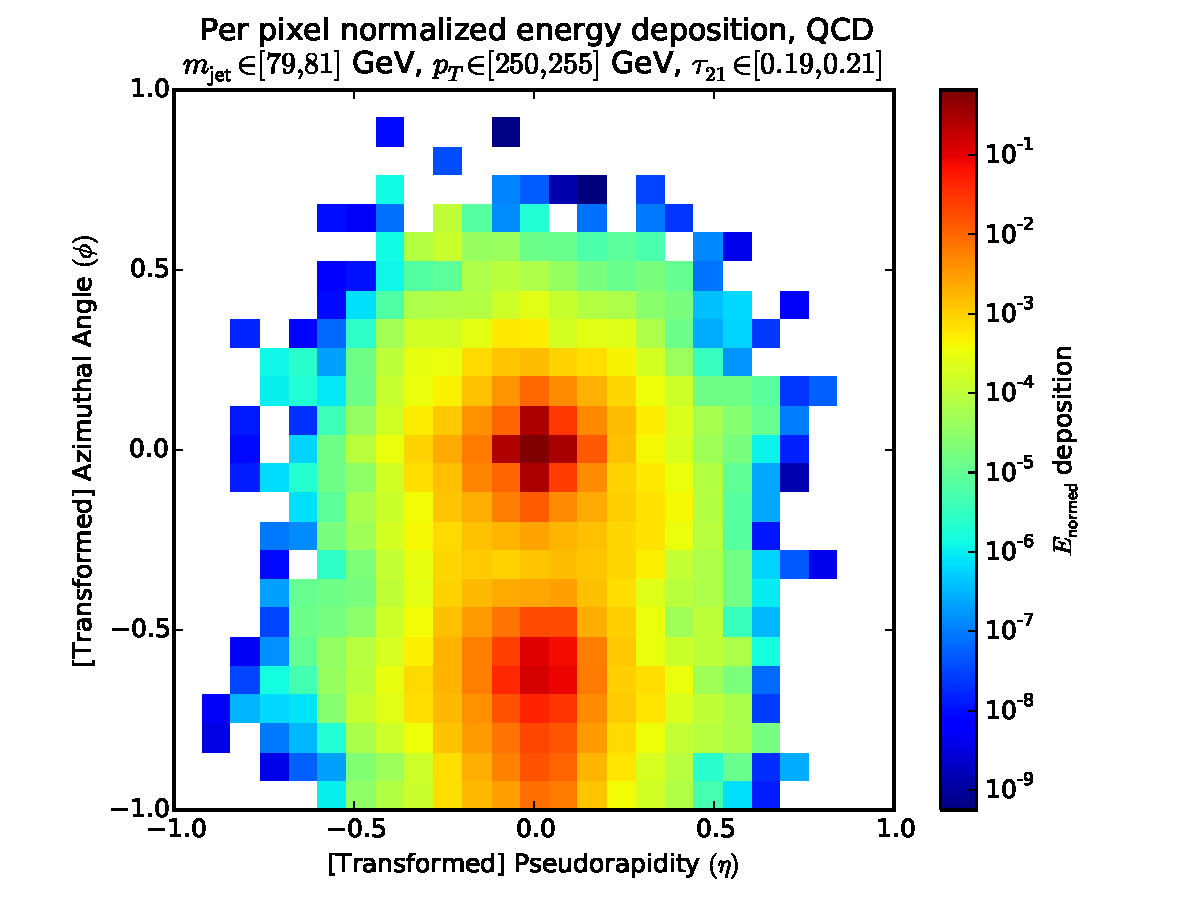
\includegraphics[width=0.5\textwidth]{figures/avg-benwindow-bkg.pdf}
      } \\
      \subfloat[Average image difference \label{subfig:windowdiff}]{
        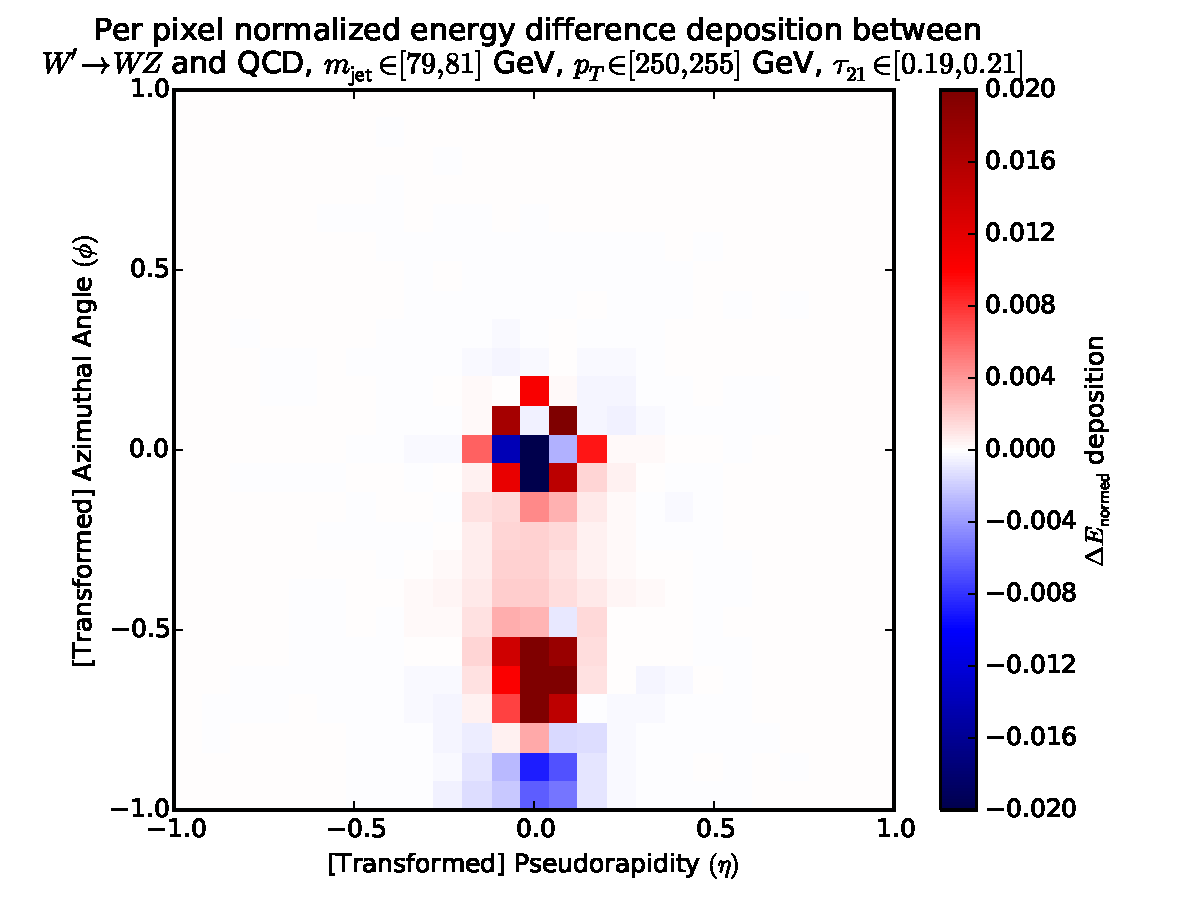
\includegraphics[width=0.5\textwidth]{figures/avg-benwindow-diff-clipped.pdf}
      }
      \caption{
        $W'\rightarrow WZ$ (left) and QCD (right) average jet-images, and Signal - Background image difference (bottom)
        \label{fig:meanImagesWindow} 
      }
    \end{center}
\end{figure}  


In this window, we compare the DNN trained outside the window to a Fisher Linear Discriminant trained inside the window. In Figure~\ref{fig:rocWindow} we see this performance comparison, and note that our DNN outperforms the FLD.

\begin{figure}[htbp]
  \centering
  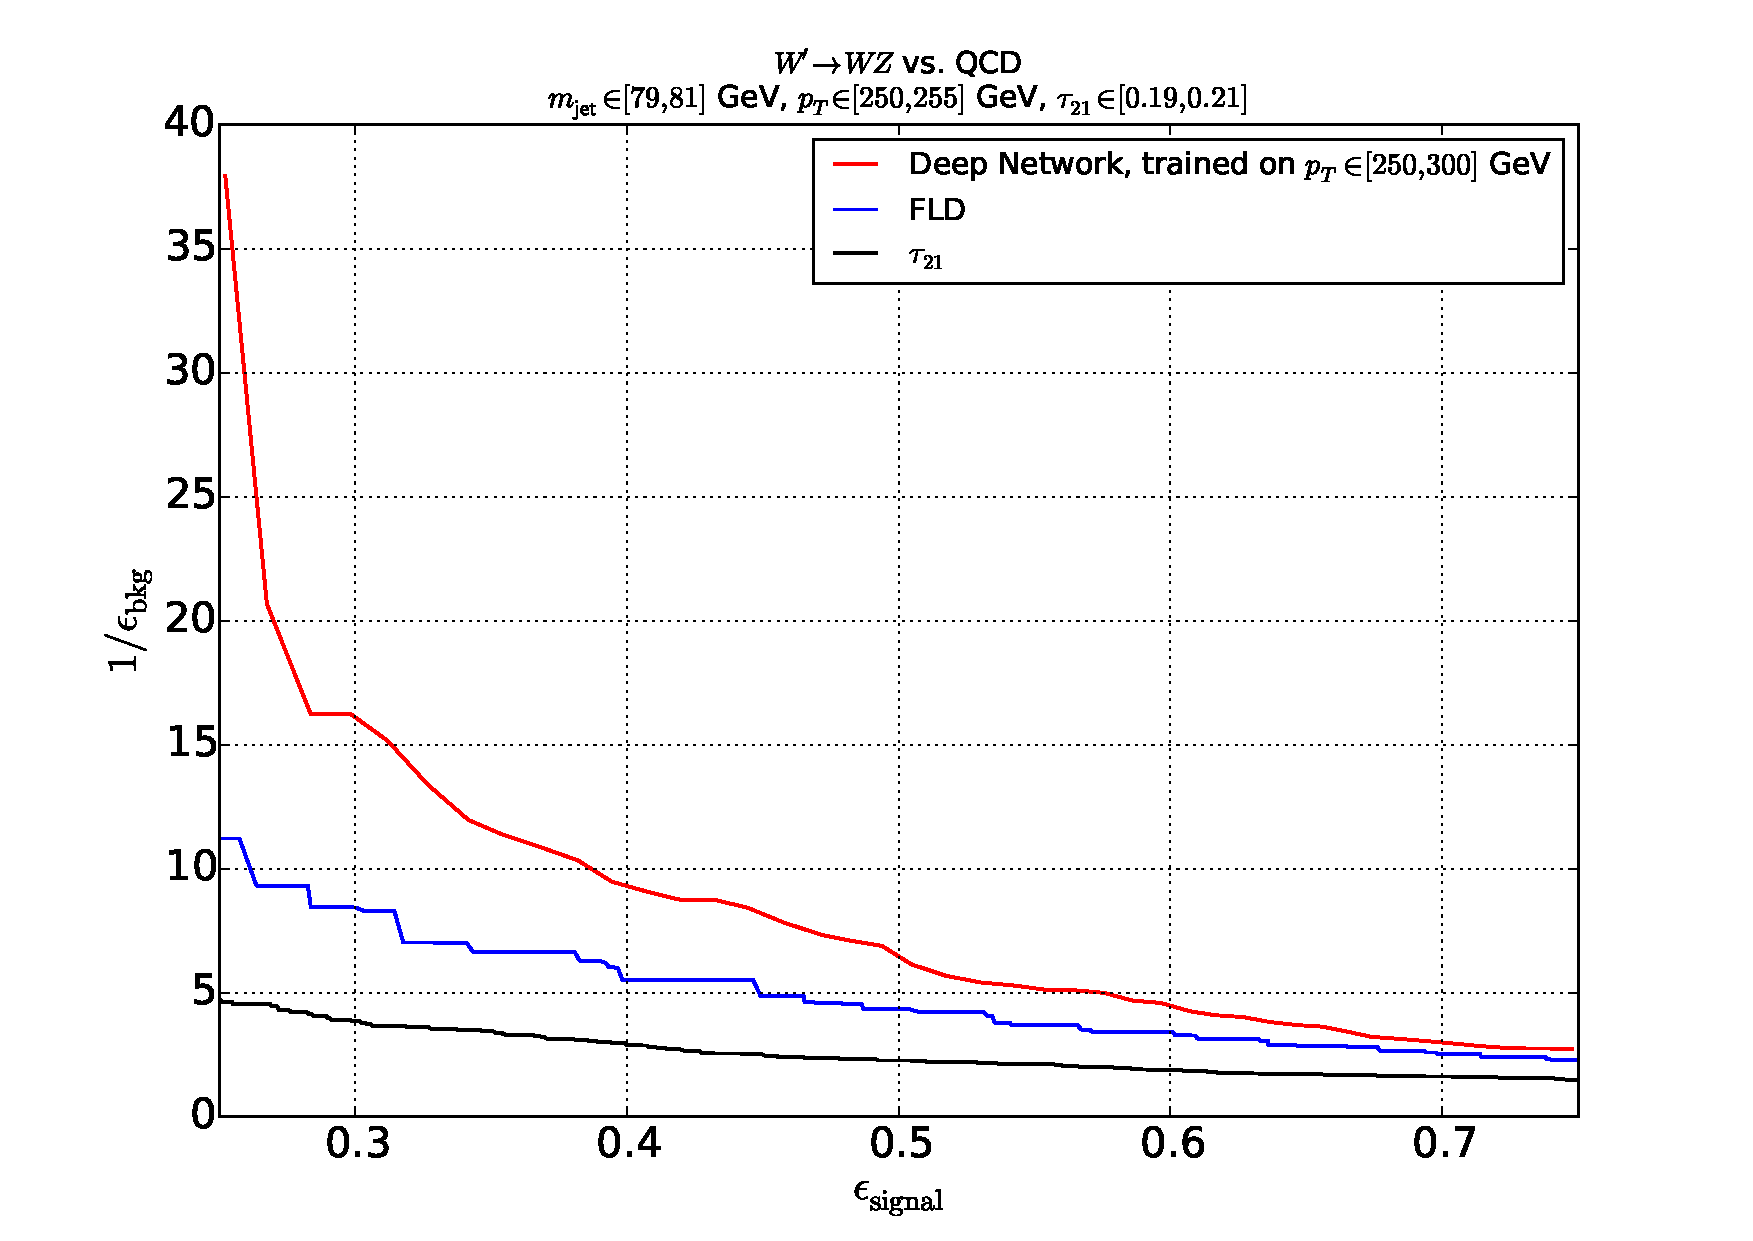
\includegraphics[width=0.95\textwidth]{figures/augwindow-roc.pdf}
  \caption{Receiver Operating Characteristic (ROC) over window sample}
  \label{fig:rocWindow}
\end{figure}

\subsubsection{Understanding what we learn} % (fold)
\label{ssub:understanding_what_we_learn}

\begin{figure}[htbp]
  \centering
  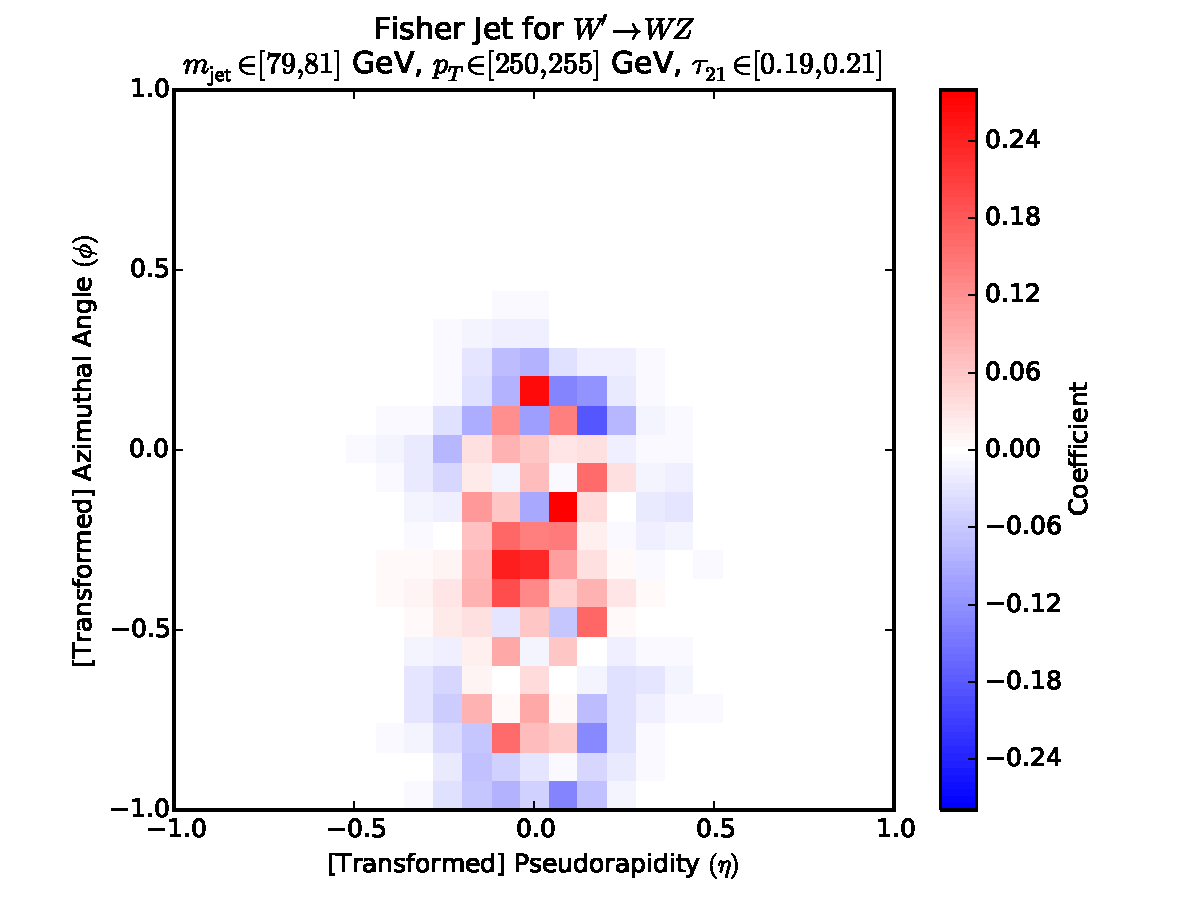
\includegraphics[width=0.65\textwidth]{figures/fld-benwindow.pdf}
  \caption{Cell coefficients from Fisher Linear Discriminant in window: $m_\text{jet}\in [79, 81]$ GeV, $p_{T}\in [250, 255]$ GeV, $\tau_{21}\in[0.19, 0.21]$}
  \label{fig:fldWindow}
\end{figure}

\begin{figure}[htbp]
  \centering
  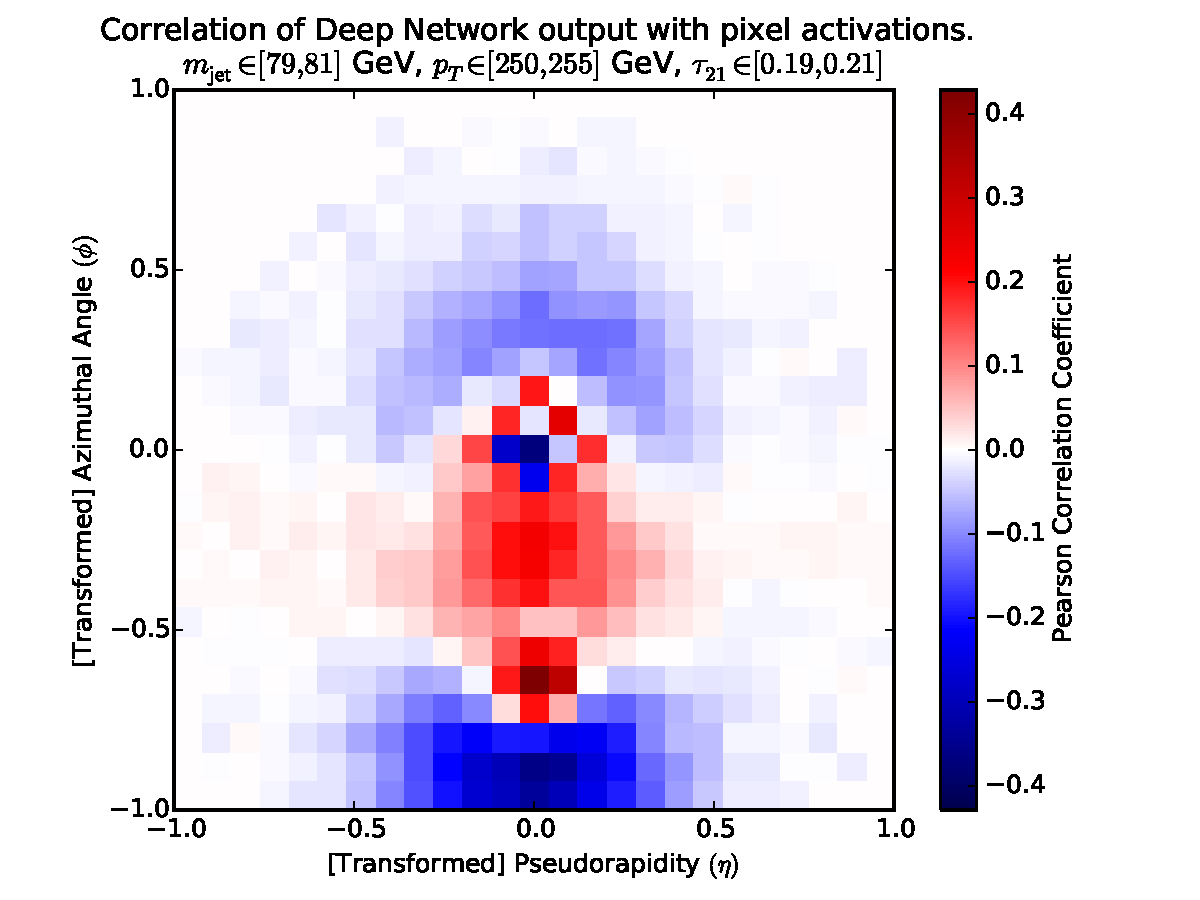
\includegraphics[width=0.65\textwidth]{figures/pixel-activations-corr-benwindow.pdf}
  \caption{Pearson Correlation Coefficient for pixels vs. DNN output, $m_{\mathsf{jet}}\in [79, 81]$ GeV, $p_{T}\in [250, 255]$ GeV, $\tau_{21}\in[0.19, 0.21]$}
  \label{fig:corrWindow}
\end{figure}

In Figure~\ref{fig:convkernelsWindow}, we show the same feature representations as in Figure~\ref{subfig:convolvedfilters}, which show the convolved differences in images over signal and background in the window. 

\begin{figure}[htbp]
  \centering
  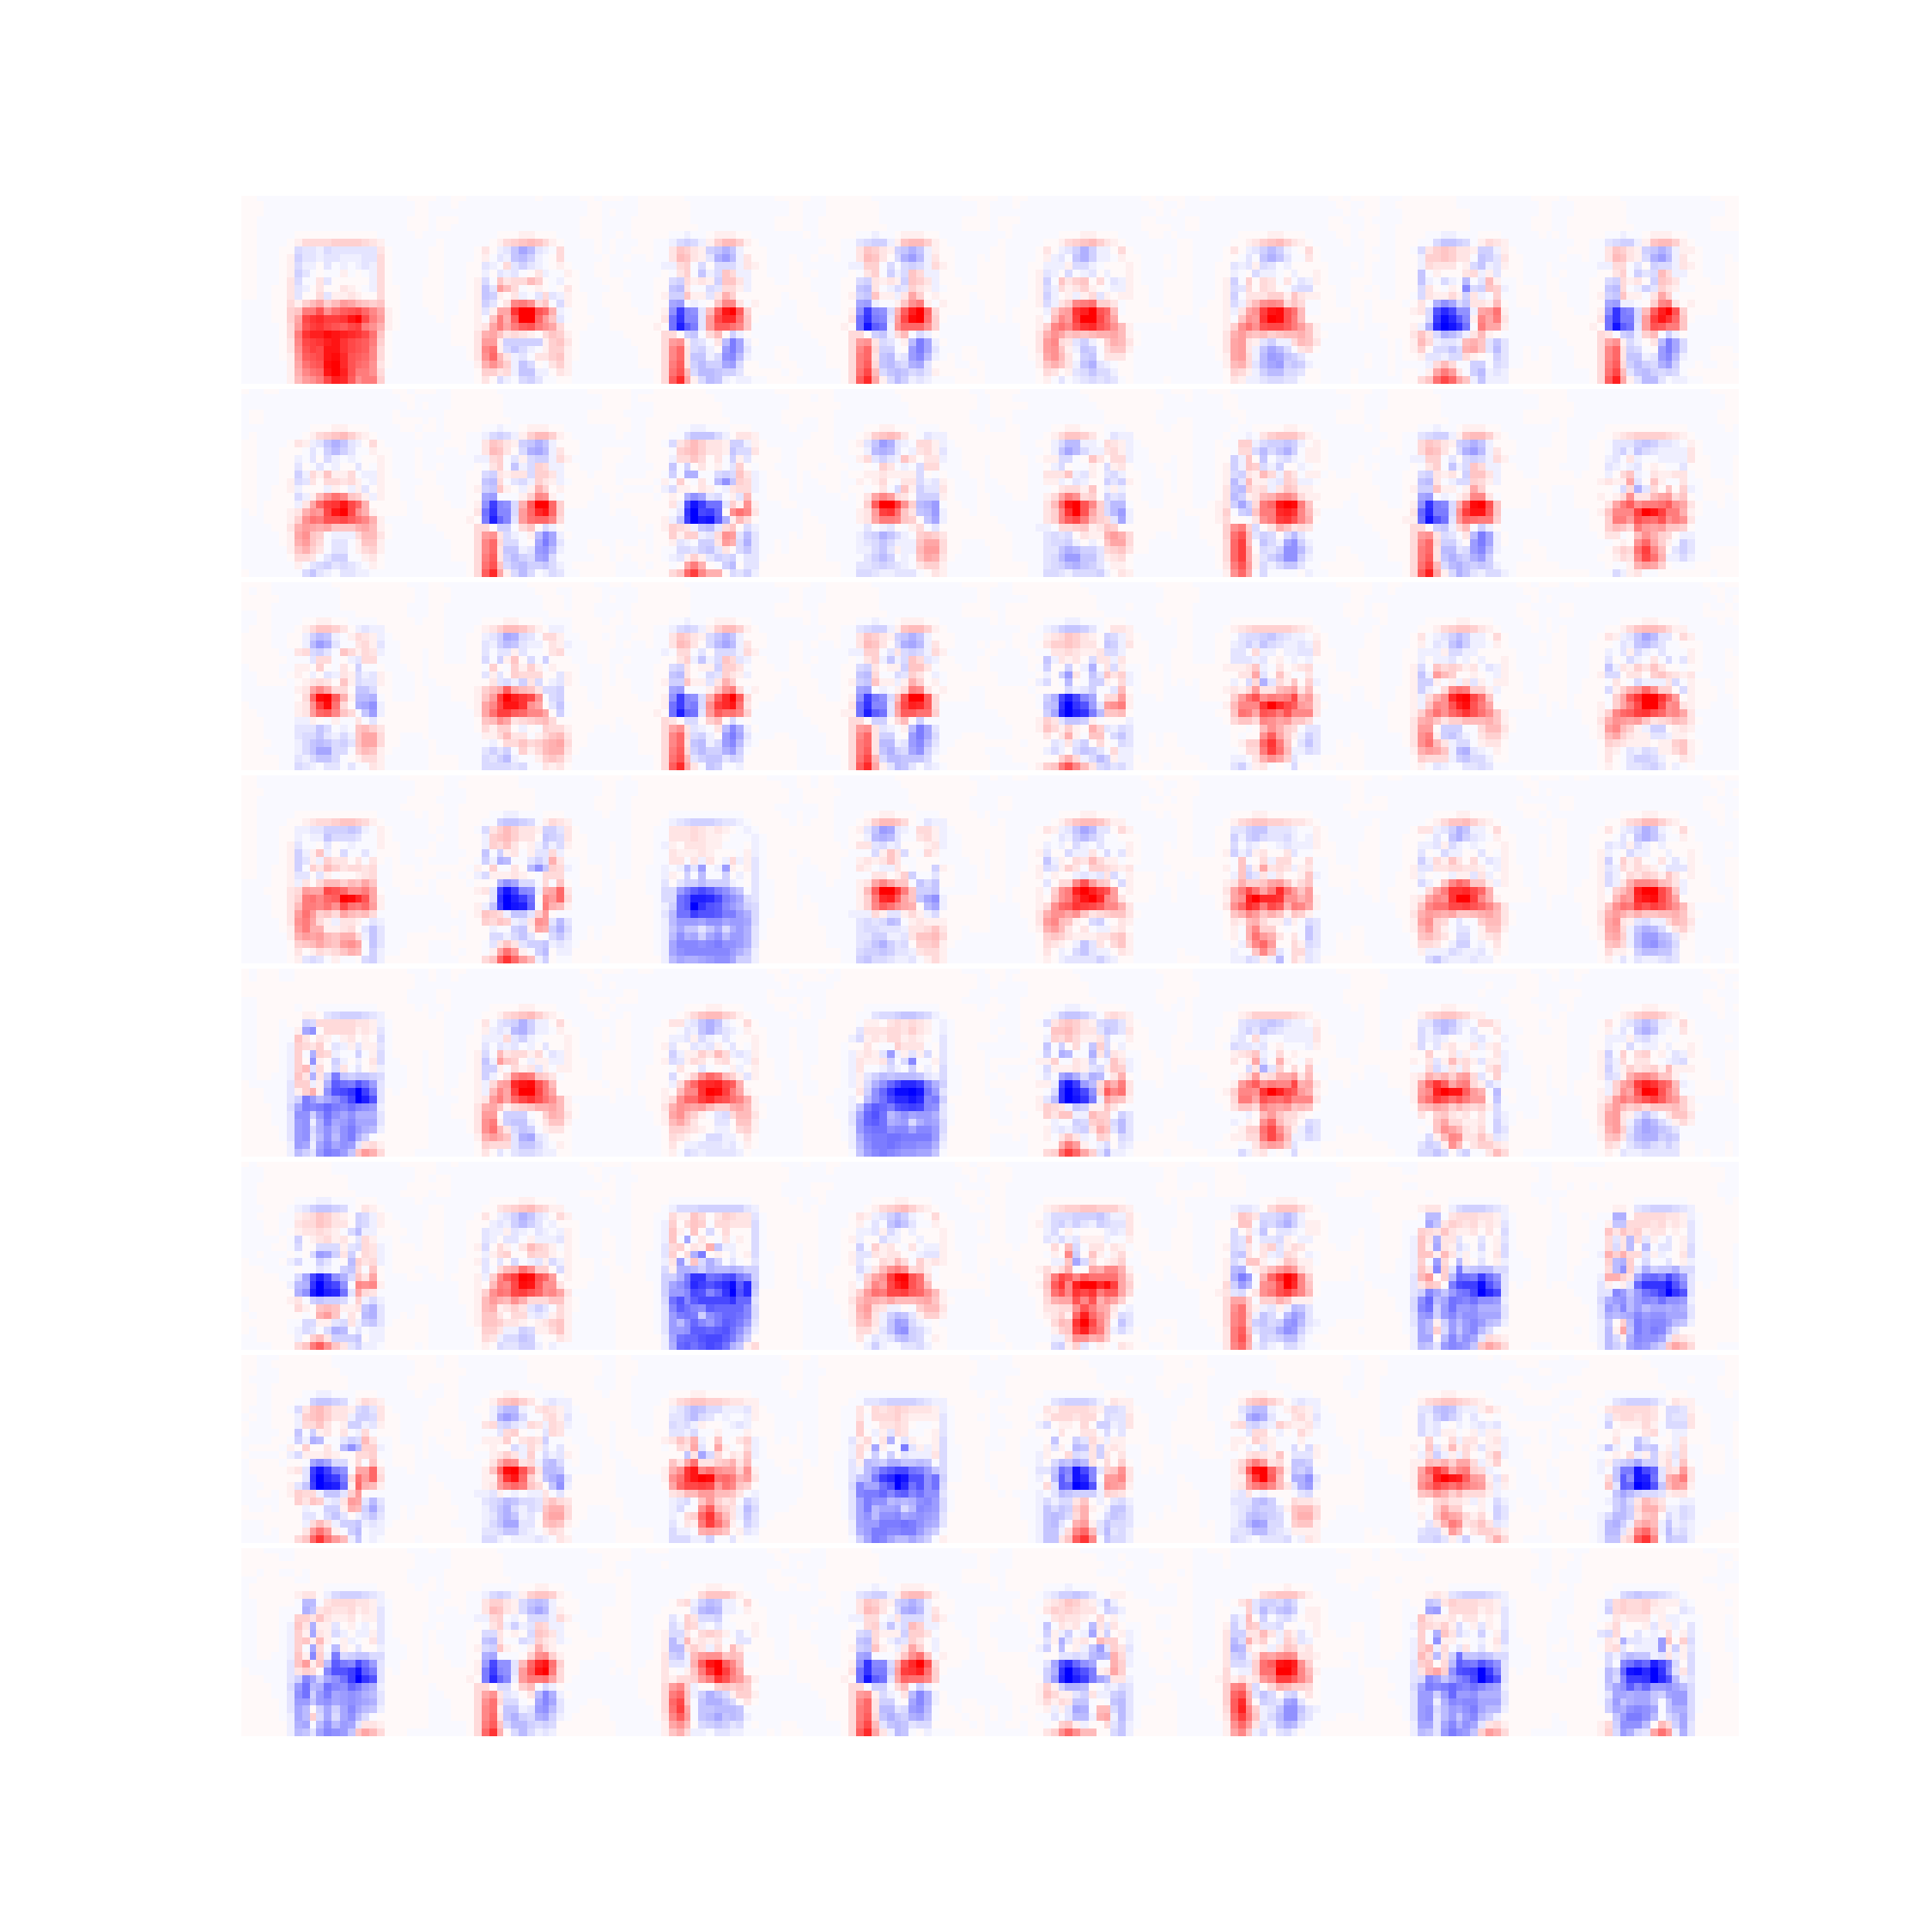
\includegraphics[width=0.95\textwidth]{figures/conv-diffs-ben-window.pdf}
  \caption{Convolved Feature Differences in jet images, $m_\text{jet}\in [79, 81]$ GeV, $p_{T}\in [250, 255]$ GeV, $\tau_{21}\in[0.19, 0.21]$}
  \label{fig:convkernelsWindow}
\end{figure}
% subsubsection understanding_what_we_learn (end)

% subsection small_window_studies (end)





% section studies (end)
